%!TEX root = ../report.tex

  \chapter{ State of the Art }

  Given the variety of different approaches to for implementing a spatio-temporal
  world model, the methods have been divided into groups. Most spatio-temporal
  world models are implemented on top of preexisting world modeling techniques
  and are therefore tied to a specific spatial
  representation. There are exceptions to this, however, with some models
  being built from the ground up, intertwining spatio and temporal components.
  Conversely, there also exists a few
  methods that can be used in conjunction with any preexisting world model. \\


  \section{ Map Dependent Models }

  \subsection{ Occupancy Grids }

  Occupancy grids were first introduced in 1985 by Moravec and Elfes. \cite{Elfes1985}
  In simple two-dimensional terms, they can be thought of as a grid placed
  over an environment. Each cell then represents the probability or belief that
  a given cell is either occupied or free. Free, in this case, meaning
  that a robot would be able to traverse through that cell. This concept can of
  course be extended into the third dimension for a more complex world model. \\

  \subsubsection{ Temporal Occupancy Grids }
  One of the earliest and most straightforward attempts to introduce a temporal
  component was to extend the existing world model in question, occupancy
  grids in particular. This can be seen in ``Temporal Occupancy Grids: a Method for
  Classifying the Spatio-Temporal Properties of the Environment''.
  \cite{Arbuckle2002} In this paper Arbuckle et al introduce the concept of
  ``temporal occupancy grids'' (TOGs). The authors noted that the key to these TOGs
  was that they "can differentiate between different patterns of occupancy, even
  when the absolute probability of occupancy is the same." That is to say, one
  could imagine a parking lot where it would be possible with TOGs to distinguish
  between cells that are parking spaces, cells that are pathways, and cells that
  are not for driving at all, such as a median. These TOGs also made it
  possible to detect where a door or elevator may be. \\

  Temporal Occupancy Grids were developed by generating multiple occupancy
  grids with contemporary methods but each occupancy grid
  would represent, and be generated using samples from, multiple different timescales.
  With multiple occupancy grids spanning multiple timescales, the
  probability of a cell being occupied could be computed by a simple summation. \\

  \subsubsection{ Hidden Markov Models }

  Hidden Markov Models (HMMs), are a type of Markov Chain that can be considered
  "a doubly embedded stochastic process with an underlying stochastic process
  that is not observable (it is hidden), but can only be observed through
  another set of stochastic processes that produce the sequence of observations."
  \cite{Rabiner1989}. Simply put, an HMM can be thought of as having N
  number of states S, that are hidden, or otherwise not directly observable.
  Each state can have M number of observations made about the properties of that state which
  may reflect indirectly, and to varying degrees of certainty, the actual state.
  Furthermore, each one of these states has a given probability distribution of
  transitioning from one state to another. It is from this information that a
  Markov Model or Markov Chain can be constructed. \\

  In the specific case of occupancy grids, each cell can be thought of as having two
  states, either free or occupied. It is not feasible to directly observe
  every given cell at all times, or more specifically, at the time of path planning.
  Thus their states are considered hidden. However, through past
  observation and data collection, a cell's data can be considered to be known
  throughout time. Thus, this temporal data can be thought of as observational data and
  can be used to make predictions about state transitions. \\

  Early combinations of HMMs with occupancy grids differed from previous dynamic
  world modeling approaches as this approach "does not depend on dynamic object
  detection and high-level object models; it considers only the occupancy of the
  space at a lower level of abstraction"\cite{Meyer-Delius2012}. By relying on
  and collecting lower, more easily observable data, larger amounts of data could
  be collected and processed over greater periods of time. Since each cell is
  dependent only on previous observations of that cell throughout time, the
  increase in data availability and the discrete nature of the predictions led to
  improved state predictions. \\

  Building on this wok, Meyer-Delius \cite{Meyer-Delius2012} introduced the concept of online
  learning to the HMM approach. Traditionally, offline learning has been used when
  a robot's navigational system would hold copy of a world model produced some
  time before operation. It is, however, possible that objects in the robot's
  environment may have changed between the time the map was generated to the
  time at which the robot operates. With the introduction of online learning, the
  robot would be able to observe these changes and factor them into its existing
  navigational system. This was the first development that attempted to surpass the static
  nature of the transition states of the HMM model. \\

  A further improvement to occupancy grids with HMMs came with the introduction of
  being able to model trajectories of the objects in an environment
  \cite{Wang2015}. Although early work on this concept was done without the use of HMMs
  \cite{Kucner2013}, newer techniques to the same end have been developed using HMMs.
  This new approach was an important improvement because the
  dynamic motion of objects in an environment, such as humans walking in a
  hallway, could now be better modeled. This process was dubbed ``Input-Output
  HMM'' (IOHMM) due nature of how cells in the grid would communicate with one
  another. Each cell would look through it's own historical data, but would
  also communicate with its neighbors. In effect, this allowed
  a cell in hallway to be able to predict occupancy based off of a nearby cell
  that is currently occupied as well as its historical occupation. This is particularly
  well suited for the prediction of trajectories and resulting cell occupation. \\

  \subsection{ Spatio-Temporal Hilbert Maps }

  \begin{figure}[!htb]
    \centering
    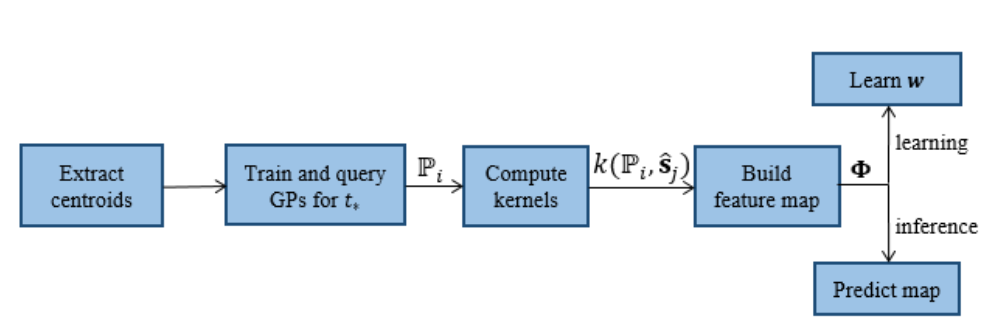
\includegraphics[width=\linewidth]{images/STHM_diag.png}
    \caption{Spatio-temporal Hilbert map training process (GP - Gaussian Process)}
    \cite{Senanayake2016}
    \label{figure:STHM}
  \end{figure}

  In contrast to the discrete nature of occupancy grids, Hilbert maps provide a
  continuous representation of an environment which allows for arbitrary world
  model resolution. They rely on "fast kernel approximations that project the
  data in a Hilbert space where a logistic regression classifier is learnt".
  A stochastic gradient optimization can then applied. This approach is similar to
  that of a Gaussian processes occupancy map but with a much lower computational
  cost. An example
  of the training process workflow is visible in figure ~\ref{figure:STHM}.
  A new development as of 2016, Hilbert maps with the addition of a temporal
  component are a new field of research, to which the authors of
  the original paper are still contributing. \cite{Ramos2016, Senanayake2016} \\

  In static Hilbert maps, the kernel can be thought of as the location of an
  obstacle or object. When introducing the temporal dimension, the centroid of a
  moving object is extracted from raw data over time. This data can the be used
  and trained on to create a model that can predict both the direction and speed of an
  object at a given location at a given time. It is particularly well-suited to
  short-term predictions such as car traffic on a road or at an intersection.
  \cite{Senanayake2016} \cite{Senanayake2017} \\

  \section{ Map Independent Models }

  \subsection{ Multi-Map Approach }
  A map-independent approach was introduced by Biber, et. al. in the mid-2000s.
  Elaborating on earlier work ``Temporal Occupancy Grids: a Method for
  Classifying the Spatio-Temporal Properties of the Environment''
  \cite{Arbuckle2002} In their paper ``Dynamic Maps for Long-Term Operation of Mobile Service Robots''
  the authors describe a method for predicting and anticipating changes in
  a dynamic environment to improve localization and navigation. This was done
  by maintaining multiple maps of a given area with each map
  being updated at a different time scale. Specifically, each cell in an occupancy
  grid, or each edge in a graph would have an author determined number of maps
  associated with it. In the paper, the example uses three maps with the
  idea being a short-term, medium, and long-term memory/map of an environment.
  Each of these maps was given a set number of observations, e.g. 20. When
  the desired number of observations have been made, all the maps are updated. During the process when
  an update happens, a certain number of observations are selected at random to
  remain and the map prepares for the next set of observations. The number of these
  observations to remain, sometimes referred to as the update ratio, determines
  what timescale a map will model. Maps keep very few observations are said to
  act like a ``short-term memory'' with ``long-term memory'' maps maintaining most of
  their observations during updates. This allows a single map to be chosen at a given
  time or for multiple maps to be averaged together depending on the desired behavior. \\

  This method's primary benefits are the simplicity of design and the ability to
  customized and tuned while working, regardless of pre-existing map
  implementations. Unfortunately, there are many parameters that need
  to be tuned. Tuning parameters can be a tedious and time consuming process.
  Additionally, parameters that work well for one problem may not work well for
  another. Finally, the authors note that the method for selecting
  the correct map is not an easy problem and often depends on the environment
  encountered and the data collected. \\


  \subsection{ FreMEn }

  Frequency Map Enhancement, or FreMEn as it became known, is a technique for
  spatio-temporal world modeling that can be used independent of mapping or
  world modeling technique. Introduced by Tomáš Krajník, Jaime Pulido
  Fentanes, Grzegorz Cielniak, Christian Dondrup, and Tom Duckett in 2014. Its
  original aim was to improve mapping for long-term scenarios.
  They observed that many previous approaches focused on mapping multiple
  static environments over time, which suited slow-changing environments, but
  may not work well for dynamic settings. In response to these issues, the
  program's original goals were to improve mapping for long-term scenarios and
  to generate mapping for highly dynamic environments. FreMEn was designed to
  resolve these issues. \cite{Fentanes2014} Although FreMEn was initially used with
  octomaps, three-dimensional occupancy grids, it was later decoupled from
  this mapping technique allowing it to be an extremely diverse and flexible
  technique. \\

  In its original and most basic form, FreMEn assumes that an environment can be
  broken down into multiple independent components. It is then further assumed
  that these independent components will take one of two binary states. Examples
  of this include a door being open or shut or a cell in
  an occupancy grid being either free or occupied. Each of these states can not
  always be directly observed, and the tools e.g. sensors available to the robot
  my have noise and cannot be taken as one hundred percent accurate. Thus,
  each component has a certain probability assigned to it. This
  probability defines the likelihood of that component being in a given state, e.g. a door
  open or closed. Finally, since these states can be observed multiple times
  over a given period, their probabilities can be defined as
  functions dependent on time. \\

  At the heart of FreMEn lies a well-known mathematical tool commonly used for
  signal processing, the Fourier Transform. Since FreMEn focuses on long-term
  observations of dynamic, often human, environments, it is assumed that harmonic
  patterns will develop over time. The Fourier Transform can then be applied to
  these long-term observations to convert them into the spatial domain for
  storage. Furthermore, because the Fourier Transform is reversible
  using the inverse Fourier Transform, one can easily convert between the stored
  observations in the spatial domain back to the time domain. This allows for
  predictions at any given time t. Not only is this extremely useful for future
  predictions, but this method can also be used to analyze the accuracy of the
  model by comparing previously observed data from the past to the model's
  predictions. Using this historical accuracy, one can then tune the order of the
  spatial model to obtain more accurate historical predictions with hopes of
  also having more accurate future predictions. More information on this process
  can be found in the original paper\cite{Fentanes2014} and the follow up FreMEn
  paper \cite{Krajnik2015}. \\

  \subsubsection{ Improvements and Additions }

  As ground breaking and flexible as FreMEn is, due to the many assumptions
  it makes, it is not without its flaws. One major assumption made is that areas of
  observation will be observed not only frequently but periodically in the most
  strict sense. That is to say, it is not only important that a location be
  visited and observed, but that the observations follow a pattern of equally
  spaced and timed observations. This is due to the Fast Fourier Transform (FFT)
  technique that is used in the original papers. To address this, later authors devised and
  implemented other methods of storing data and making predictions. These methods often
  involve phase shifting or modifying the amplitude of the observation as well
  as using a modified equation derived from the Fourier Transform instead of the
  standard FFT. More information can be found in the paper \cite{Santos2016}. \\

  Another major limitation of FreMEn is its assumption that all observable
  behavior can be modeled with binary states. One attempt at solving this issue
  involves replacing the Bernoulli distribution of FreMEn with a Poisson base approach.
  The aim of this being to
  better represent human patterns present in environment such as
  an office building or hospital. Specifically, they "extend the technique
  (FreMEn) by employing both Poisson processes as the counting model to replace
  the binary states of FreMEn and a new way of selecting the most prominent
  frequency components of the Fourier spectrum."\cite{Jovan2016} This approach,
  however, does not come without its own set of assumptions and problems. By
  using a Poisson process instead of a Bernoulli distribution predictive models are no longer
  limited to binary states, but because a probability mass distribution is used
  the primary factors are $\gamma$ and N. $\gamma$ being the average number of
  occurrences of an object or behavior in a fixed time and N being the actual
  number of occurrences in a given time frame. These factors limit this
  approach to only being able to estimate objects or behaviors that are
  countable. This would not work well for something like predicted travel time,
  for instance. \\

  In the same paper,
  ``A Poisson-Spectral Model for Modelling Temporal Patterns in Human Data Observed by a Robot``
  \cite{Jovan2016}, another interesting modification was made. In order to mesh
  the Poisson Process with the observed month long data and also
  increase confidence, the data was broken into week-long segments and then
  stacked on top of itself. The thought behind this is that it not only
  increase the number of data points to train on, but also accounts for behaviors in human
  environments that can often be cyclic on week boundaries. Although this works well
  assuming all behaviors happen with weekly periodicity, it is not always
  the case, and thus behaviors that don't occur every seven days at the same time
  may be incorrectly predicted. An example of a weeks worth of data is visible
  in figure ~\ref{figure:PSP}. \\

  However, this idea of manipulating and folding observed data over itself through time
  continued to evolve. Recently, in
  ``Warped Hypertime Representations for Long-term Autonomy of Mobile Robots''
  \cite{Krajnik2018} the idea was taken a step further. This paper, continues
  to build off of FreMEn, using the same Fourier-like approach to observing
  periodicity in a data set. It continues to build off of the ideas mentioned
  in \cite{Jovan2016}. Now, no longer is data restricted to being folded at a
  single point, instead, it is folded back on itself at one of many possible
  frequencies. When and where to fold the data is determined using one of two
  recommended methods. Either expectation maximization or K-means clustering.
  The processes of finding when and where to fold is iterative and the number
  of folds, which can be thought of as the order, can be either hard limited
  or determined during training when the error introduced by increasing the
  order is greater than that of the previous step. This approach not only allows
  for non-binary predictions of any data observation type, but also
  for sparse or infrequent data to be the basis of prediction, due to the
  folding of the data. \\



  \begin{figure}[!htb]
    \centering
    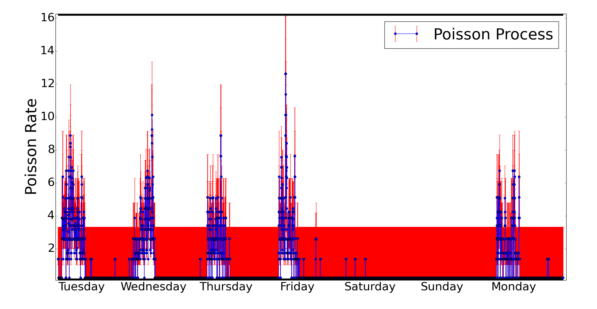
\includegraphics[width=\linewidth]{images/poisson-spectral-process.png}
    \caption{Lambda time series of a corridor using Poisson Process}
    \cite{Jovan2016}
    \label{figure:PSP}
  \end{figure}


  \section{ Existing Methods for Evaluation or Comparison }

  It is clear that there are a multitude of different methods for doing
  spatio-temporal world modeling. Given this range of methods available
  there has been an initial push to create a means of evaluating and comparing methods
  with other approaches. The vast majority of these evaluations look internally,
  comparing a given method with a fixed set of parameters with the same method with
  the parameters slightly varied from the original. Yet others, although fewer
  in number, do set more general criteria that can be directly used or extended
  to evaluate their performance with respect to any other spatio-temporal
  world modeling technique. Because methods for comparing a model against itself
  with different parameters can often be very specific, this section will focus
  on those existing methods that have been, or can be, extended to allow any
  modeling method to be compared to another. \\

  \subsection{ Current Methods and Limitations}

  \subsubsection { Prediction Accuracy }
  Arguably the most obvious and most used metric for comparing spatio-temporal
  world modeling techniques is to compare the accuracy of a prediction
  to the ground truth over time. In the case of binary data, for example in
  ``Occupancy Grid Models for Robot Mapping in Changing Environments'',
  \cite{Meyer-Delius2012} the accuracy of an occupancy grid map is evaluated as
  a whole over a discreet number of time steps. For a given time step t,
  each cell in the grid is compared to a ground truth value. These are then
  summed up to produce an average accuracy at a given time t and plotted over
  time. These were used to compare different maps produced by the same algorithm
  but with different parameters. ``Spatio-Temporal Hilbert Maps for Continuous
  Occupancy Representation in Dynamic Environments'' \cite{Senanayake2016}
  takes this a step further and advances this method by comparing variations
  both forward and backward in time. This allows for further
  improved training and adjusting tested technique's parameters. Finally,
  ``Learning Temporal Context for Activity Recognition'' \cite{Coppola2016}
  extended this method for comparison to be used to compare multiple different
  spatio-temporal world modeling techniques over multiple days worth of data. \\

  \subsubsection { Resource Usage }

  One extremely relevant method that is often used in other fields of study
  is a comparison of run-time usage of computational resources. This is even
  more pertinent when one considers the effect spatio-temporal world models may
  have on a system when deployed to a real-world environment. This is especially
  important when the ability to scale is required. Unfortunately, there is currently
  no standard technique for collecting or comparing this data.
  Perhaps one of the only examples of a discussion of run-time resource usage
  appears in ``Spatio-Temporal Hilbert Maps for Continuous Occupancy Representation in Dynamic Environments'' \cite{Senanayake2016}.
  Sadly, this is only gives a rough estimate, on the order of a half second,
  that an average single observation and prediction would take. Moving forward
  it would be desirable to have not only detailed observations of run-time
  memory and processor usage, but also a comparison of resource usage with
  respect to the multiple techniques being compared. \\


\end{document}
